%%
%% licence       kaneton licence
%%
%% project       kaneton
%%
%% file          /home/buckman/kaneton/view/book/assignments/2007/k4/k4.tex
%%
%% created	 pidancet julian	[tue may29 16:34:56 2006]
%% updated	 pidancet julian	[tue may29 16:34:56 2006]
%%

%
% k2
%

\chapter{K4: IPC Management}

%
% informations
%

\begin{tabular}{p{7cm}l}
Duration: & 2 weeks \\
Directory name: & kaneton/ \\
In charge: & Julian Pidancet, Matthieu Bucchianeri \& Renaud Voltz\\
Mailing-list: & kaneton-students@googlegroups.com \\
Languages: & C, assembly \\
Students per group: & 2 (same groups as for K3) \\
\end{tabular}

\section{Abstract}

K4 project consists in developing the last part of the microkernel :
the IPC (Inter-process Communication). As you know, in a microkernel,
contrary to a monolithic kernel, every kernel services are running
independently from the core, in separate userspace tasks. In order to
communicate, tasks need to interact : sending, receiving messages, and
also synchronizing each others. The IPC model chosen for kaneton is
``message passing''.

The concerned parts are:

\begin{enumerate}
  \item
    {\bf The message manager, messaging primitives (1)} \\
    Inter-process messaging primitives. Send and receive functions,
    synchronous and asynchronous.
  \item
    {\bf The message manager, IA-32 Syscall Handlers (2)}\\
    Handling kernel side soft-interrupts (syscalls to the messaging
    primitives).
  \item
    {\bf Task side, IA-32 Syscall Triggers (3)}\\
    Userland syscall functions (sends soft interrupts to the kernel to
    send a message from userland).
\end{enumerate}

\begin{center}
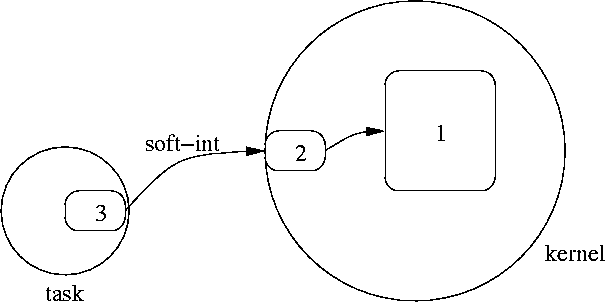
\includegraphics[width=0.5\linewidth]{figures/message.png}
\end{center}

\newpage

\section{message manager, \textbf{messaging primitives}}

\begin{itemize}
  \item {\bf Overview}\\

    This part of the code contains the 4 messaging primitives: sending
    and receiving in both asynchronous and synchronous mode.

  \item {\bf Assignments}\\

    In the machine-independant part of the message manager, you will
    have to implement the messaging primitives for sending and
    receiving messages.  These primitives will have to be accessible
    by syscalls, to permit running tasks to send and receive messages
    from userspace (see the 2 next sections).

  \item {\bf Interface}\\

\function{message\_async\_send}{(i\_task \argument{sender},
				 i\_node \argument{dest},
				 t\_tag \argument{tag},
				 t\_vaddr \argument{data},
				 t\_vsize \argument{size})}
	 {
	   \item This primitive sends asynchronously a message to the task
	   referenced by the field \textbf{taskid} of the \argument{dest}
	   parameter. (The field \textbf{machineid} of \argument{dest}
	   is ignored).

	   \item The \argument{sender} parameter refer to the sending task, this
	   parameter should be set by the kernel syscall handlers with the
	   calling task, which can be obtained by result to a call of
	   \textbf{task\_current()}.

	   \item The \argument{tag} parameter is ignored, it should be used in the
	   future to apply selection on the queued messages in a task's
	   message box.

	   \item \argument{data} designate the virtual address of the buffer to be
	   transmit. Be carreful, this address is not always mapped in the
	   kernel address space, address space of \argument{data} can be
	   retrieved in the \argument{sender}'s \textbf{o\_task}.

	   \item \argument{size} is the size of the message in the
	   \argument{data} buffer.
	 }

\function{message\_async\_recv}{(i\_task \argument{receiver},
				 t\_tag \argument{tag},
				 t\_vaddr \argument{buff},
				 t\_vsize \argument{buffsz},
				 i\_node* \argument{sender},
				 t\_vsize* \argument{msgsz})}
	 {
	   \item This primitive receive an asynchronous message and returns
	   an error if no messages are pending for the \argument{receiver}
	   task. \argument{sender} parameter refer to the receiving task,
	   this parameter should be set by the kernel syscall handlers with the
	   calling task, which can be obtained by result to a call of
	   \textbf{task\_current()}.

	   \item The \argument{tag} parameter is ignored, it should be used in the
	   future to apply selection on the queued messages in a task's
	   message box.

	   \item \argument{buff} designate the virtual address of the receiving
	   buffer to be written. Be carreful, this address is not always
	   mapped in the kernel address space, address space of \argument{buff}
	   can be retrieved in the \argument{sender}'s \textbf{o\_task}.

	   \item \argument{maxsz} is the size of the receiving buffer, used
	   to prevent buffer overflow.

	   \item \argument{sender} and \argument{msgsz} are pointers used to
	   return the sender and the size of the received message. Be carefull,
	   theses pointers are not pointers to calling task's address space,
	   the return values will have to be passed by registers while
	   returning from syscall.
	 }

\function{message\_sync\_send}{(i\_task \argument{sender},
				i\_node \argument{dest},
				t\_tag \argument{tag},
				t\_vaddr \argument{data},
				t\_vsize \argument{size})}
	 {
	   \item Send a message synchronously.

	   \item See \textbf{message\_async\_send()} for parameters details.
	 }

\function{message\_sync\_recv}{(i\_task \argument{receiver},
				t\_tag \argument{tag},
				t\_vaddr \argument{data},
				t\_vsize \argument{maxsz},
				t\_state \argument{blocking},
				i\_node* \argument{sender},
				t\_vsize* \argument{msgsz})}
	 {
	   \item Receive a synchronous message.

	   \item The \argument{blocking} parameter is a boolean which
	   set the behaviour of the function if no symetric
	   \textbf{message\_sync\_send()} to task \argument{receiver}
	   happened before. In this case, if \argument{blocking}
	   is clear, the function return immediatly an error.
	   If \argument{blocking} is set, the task \argument{receiver}
	   will be blocked until another task try to synchronize with it.

	   \item See \textbf{message\_async\_recv()} for other parameters
	   details.
	 }


  \item {\bf {Files}}\\

    \begin{tabular}{| l | l |}
      \hline
      machine-independent & {\em kaneton/core/message/message.c}\\
      &  {\em kaneton/include/core/message.h}\\\hline
    \end{tabular}
\end{itemize}

\section{message manager, \textbf{IA-32 syscalls handlers}}
\begin{itemize}
  \item {\bf Overview}\\

    This part of the code is used to hook software interrupts to your
    handlers. These handlers must read the passed argument from the
    interrupted context, call the right function of the message
    manager, and writeback results into the interrupted context.

  \item {\bf Assignments}\\

    No special model is given. You can implement the kernel-side of
    your syscalls as you want. You may use one interrupt gate per
    syscall or only one gate for all the syscalls (then adding an
    argument identifying which syscall is invoked).

  \item {\bf {Files}}\\

    \begin{tabular}{| l | l |}
      \hline
      machine-dependent & {\em kaneton/core/arch/ibm-pc.ia32-virtual/message.c}\\
      & {\em kaneton/include/arch/ibm-pc.ia32-virtual/core/message.h}\\\hline
    \end{tabular}

\end{itemize}

\newpage

\section{Task side, \textbf{IA-32 syscall triggers}}
\begin{itemize}
  \item {\bf Overview}\\

    This portion of code will be used by user (and kernel) tasks. IRL,
    it would be located in the libc (like in UN*X systems, the
    \emph{read} function that does the read syscall is located in the
    libc), but as the kernel code is always mapped to make the debug
    and testing easier, it will be put into this code.

    Each function must:

    \begin{itemize}
      \item
	Put the incoming arguments in registers
      \item
	Trigger the right software interrupt
      \item
	Get back the results from the registers to the outgoing arguments
    \end{itemize}

  \item {\bf Assignments}\\

    Implement the 4 syscalls so the userland tasks can call the
    message manager into the kernel.

    XXX

  \item {\bf Interface}\\

\function{syscall\_async\_send}{(i\_node \argument{dest},
				 t\_tag \argument{tag},
				 void* \argument{data},
				 t\_size \argument{size})}
	 {}

\function{syscall\_async\_recv}{(t\_tag \argument{tag},
				 void* \argument{buff},
				 t\_size \argument{maxsz},
				 i\_node* \argument{sender},
				 t\_size* \argument{msgsz})}
	 {}

\function{syscall\_sync\_send}{(i\_node \argument{dest},
				t\_tag \argument{tag},
				void* \argument{data},
				t\_size \argument{size})}
	 {}

\function{syscall\_sync\_recv}{(t\_tag \argument{tag},
				void* \argument{buff},
				t\_size \argument{maxsz},
				t\_state \argument{blocking},
				i\_node* \argument{sender},
				t\_size* \argument{msgsz})}
	 {See above sections}

  \item {\bf {Files}}\\

    \begin{tabular}{| l | l |}
      \hline
      machine-dependent & {\em kaneton/core/arch/ibm-pc.ia32-virtual/message.c}\\
      & {\em kaneton/include/arch/ibm-pc.ia32-virtual/core/message.h}\\\hline
    \end{tabular}

\end{itemize}

%
% appendix
%

\newpage

\section{Appendix}

\textbf{Example of messaging syscall use\ldots}

Task 1 sends ``ping'' to task 2, and task 2 answer ``pong'' to task 1.

\begin{enumerate}
  \item Using synchronous send and receive, Task 1 and task2 first
  synchronize together, the string ``ping'' is then copied directly from task 1
  address space to task 2 address space.

  \item	Then task 1 enters in a polling loop, waiting to an answer, because
  task2 answer in asynchronous mode. The string ``pong'' is copied into task 1
  address space in two times : message is queued into the kernel memory between
  the two calls.
\end{enumerate}

\begin{itemize}
  \item Task 1

\begin{verbatim}
void             tsk1_main()
{
  char          *to_send = "ping";
  i_node        dest;

  char		recv[64];
  i_node	from;
  t_size	recv_sz = 0;

  dest.task = 2;

  /* Synchronize to task 2 and send "ping" */
  syscall_sync_send(dest, 0, to_send, 5);

  /* Polling to receive a message */
  while (syscall_async_recv(0, recv, 64, &from, &recv_sz) != ERROR_NONE
         && from != 2)
    ;
}
\end{verbatim}

  \item Task 2

\begin{verbatim}
void             tsk2_main()
{
  char          *to_send = "pong";
  i_node        from;
  char		recv[64];
  t_size	recv_sz = 0;

  /* Synchronize, and receive a message */
  syscall_sync_recv(0, recv, 64, 1, &from, &recv_sz);

  /* Answer asynchronously */
  syscall_async_send(from, 0, to_send, 5);
}
\end{verbatim}

\end{itemize}
